\subsection{Testing basic ALU functions and Register File}
The first program is used to verify that the ALU is capable of carrying out all basic instructions and rewriting them in the Register File.
\begin{figure}[H]
	\centering
	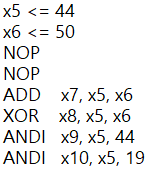
\includegraphics[width=0.2\textwidth]{sec3/images/test1.png}
	\caption{Testing ALU and Register File}
	\label{fig:test1}
\end{figure}
\noindent The first instructions initialise registers x5 and x6 to two known values, then two NOPs are inserted to avoid data hazard and finally several arithmetic operations are performed and the results saved in registers. As can be seen from \autoref{fig:wavetest1}, in registers x7, x8, x9 and x10 there are respectively sum, bitwise XOR and AND immediate, once with an identical operands and once with  different operands.\\
\begin{figure}[H]
	\centering
	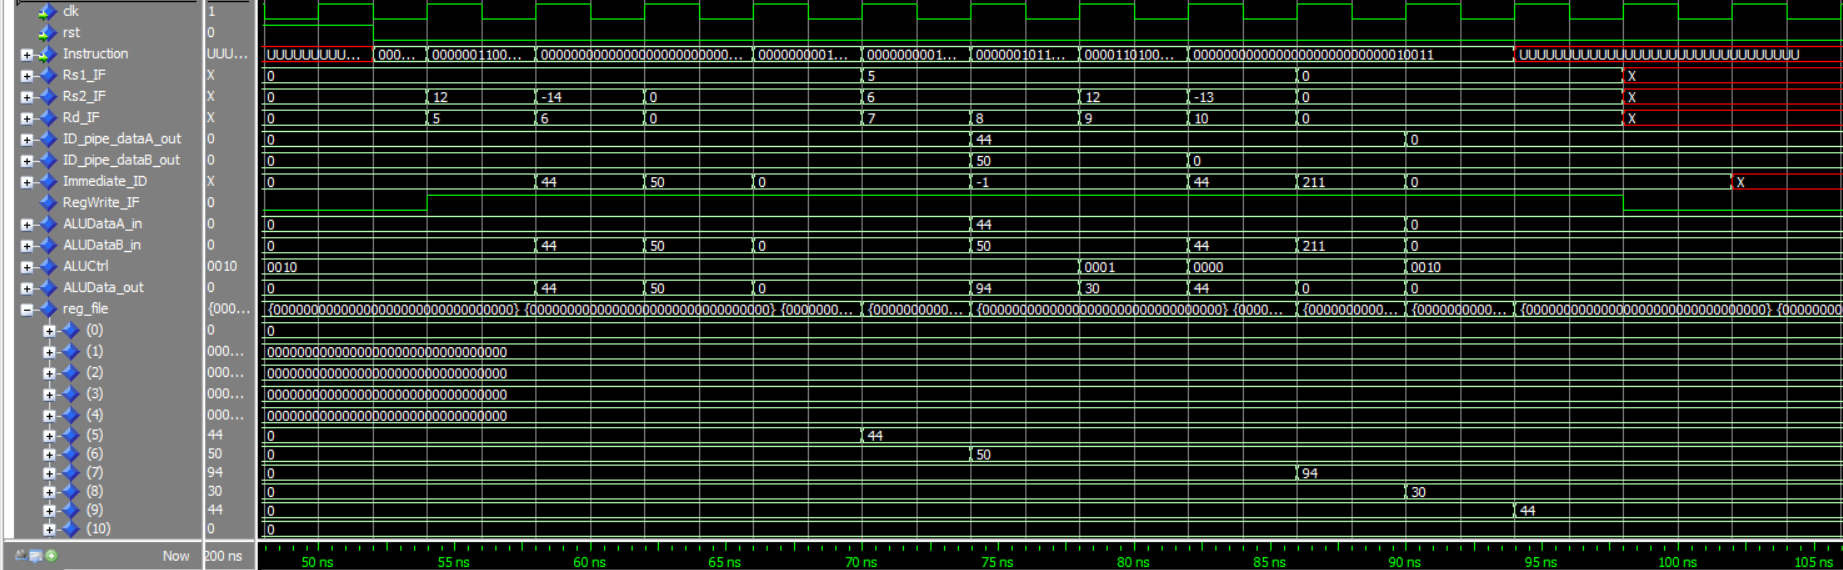
\includegraphics[width=1\textwidth]{sec3/images/wave_test1.png}
	\caption{Testing ALU and Register File}
	\label{fig:wavetest1}
\end{figure}
\noindent It can be seen that all control signals are correctly synchronised and data is written to the Register File.
\pagebreak

\subsection{Testing Data Memory}
This script aims to test the functionality of the data memory in reading and writing mode.
\begin{figure}[H]
	\centering
	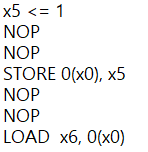
\includegraphics[width=0.2\textwidth]{sec3/images/test2.png}
	\caption{Testing Data Memory}
	\label{fig:test2}
\end{figure}
\noindent The first instruction initializes the x5 register to the value 1, after which it is stored in the memory cell pointed by x0, i.e. cell 0. Finally, a load is performed to read the same memory cell and save its content in x6.\\
As shown in the \autoref{fig:wavetest2}, in the Register file the value 1 is present both in position x5 and x6, a sign that the simulation has been successful. In addition, the memory enable signals worked correctly. In this program there were no data hazards in fact NOPs were inserted between one operation and another.
\begin{figure}[H]
	\centering
	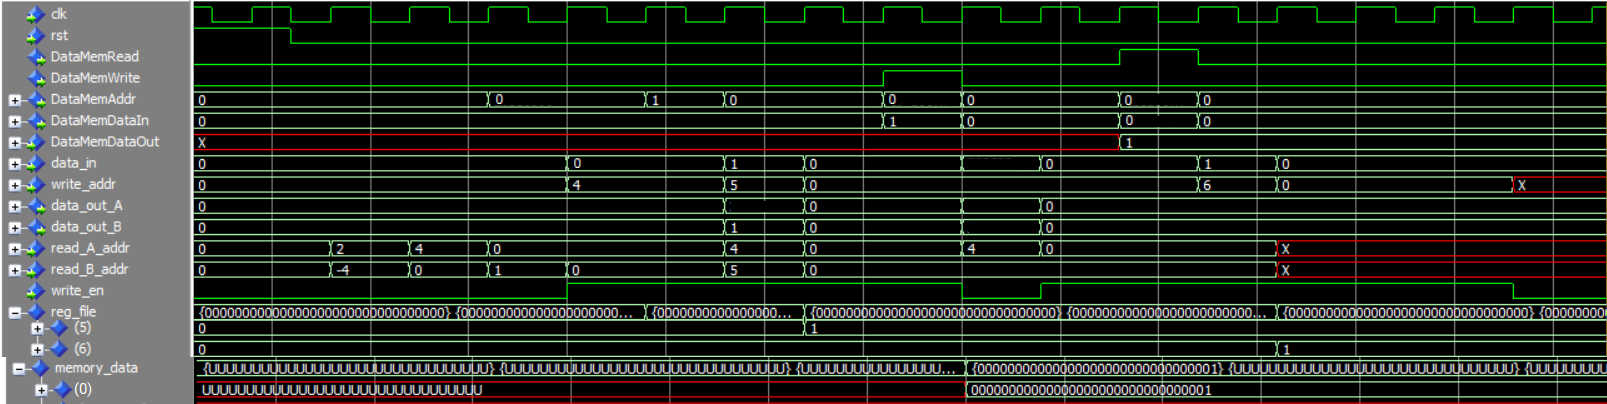
\includegraphics[width=1\textwidth]{sec3/images/wave_test2.png}
	\caption{Testing Data Memory}
	\label{fig:wavetest2}
\end{figure}

\subsection{Testing Branch instructions}
This script will test the functionality of the hazard detection unit when a jump instruction occurs.
\begin{figure}[H]
	\centering
	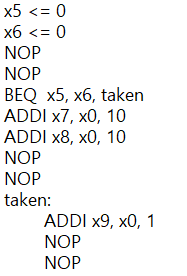
\includegraphics[width=0.2\textwidth]{sec3/images/test3.png}
	\caption{Testing branch instructions}
	\label{fig:test3}
\end{figure}
\noindent Registers x5 and x6 are both initialised to 0 to make the jump condition true. After the branch instruction, two sums are inserted to modify the contents of registers x7 and x8 in order to check that they are not actually modified. Finally, to confirm that the jump has taken place, as well as checking that the PC has been updated, it can be observed that register x9 has been updated with the value 1, i.e. the first instruction after the jump has been executed correctly.\\
As shown in the simulation \autoref{fig:wavetest3_1}, during the Execute stage the signal coming from the branch comparator becomes valid, so the pipeline registers referring to the Fetch and Decode stages are flushed and the PC is updated with the jump address. The hazard detection unit and the jumping mechanism work correctly, the overhead in case of a taken branch is equal to two instructions after which it continues sequentially starting from the jumping address contained in the branch instruction.
In \autoref{fig:wavetest3_2}, on the other hand, the x5 and x6 registers are at two different values so that the jump is not performed, therefore the x7 and x8 registers are changed.
\begin{figure}[H]
	\centering
	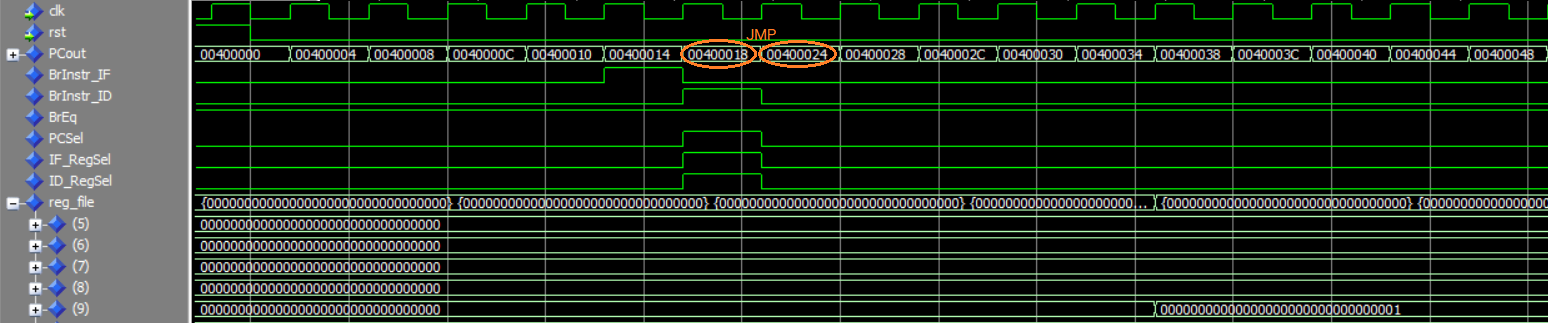
\includegraphics[width=1\textwidth]{sec3/images/wave_test3_1.png}
	\caption{Test with taken branch}
	\label{fig:wavetest3_1}
\end{figure}
\begin{figure}[H]
	\centering
	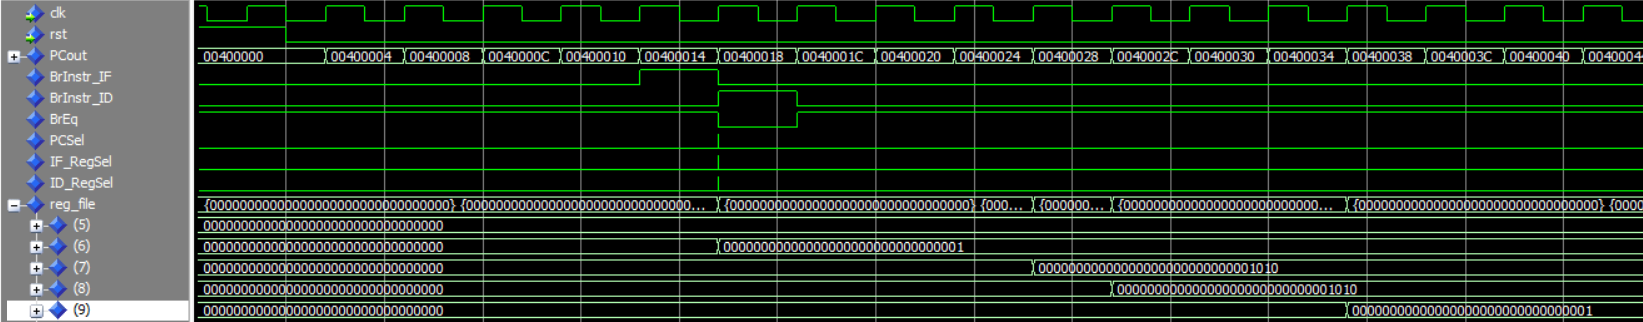
\includegraphics[width=1\textwidth]{sec3/images/wave_test3_2.png}
	\caption{Testing with un-taken branch}
	\label{fig:wavetest3_2}
\end{figure}

\subsection{Testing Forwarding Mechanism}
The purpose of these scripts is to verify that the forwarding mechanism is working correctly. 
\begin{figure}[H]
	\centering
	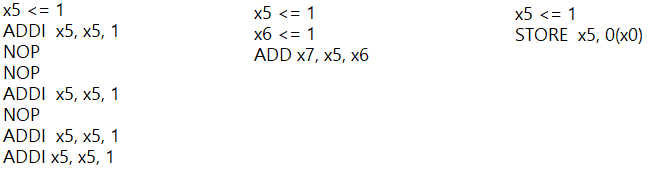
\includegraphics[width=0.8\textwidth]{sec3/images/test456.png}
	\caption{Testing forwarding mechanism}
	\label{fig:test456}
\end{figure}
\noindent In the first script there are two different situations in which a given dependency occurs, one in which the distance between instructions is equal to one clock cycle and a second in which the distance is equal to 2. The first case is solved by forwarding the ALU's output register, while the second by taking the Write Back register. From the \autoref{fig:wavetest4}, it can be noticed that the final value of the x5 register is equal to 5, that is the number of times the sum instruction has been executed, and the forwarding signal change value for each different data dependency.
\begin{figure}[H]
	\centering
	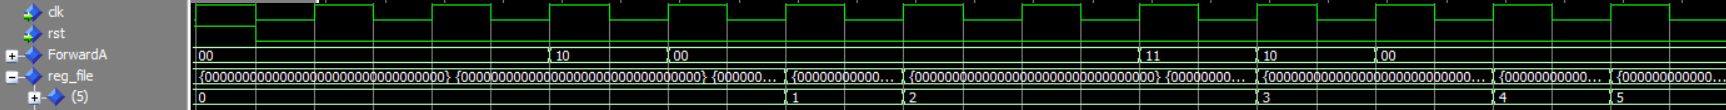
\includegraphics[width=1\textwidth]{sec3/images/wave_test4.png}
	\caption{Testing Forwarding}
	\label{fig:wavetest4}
\end{figure}
\noindent The second script aims to verify a similar case to the previous one adding a complexity factor. The add instruction requires both registers x6 and x5 whose contents have been modified at the previous clock cycle and the one before that, respectively. In the \autoref{fig:wavetest5} it can be read that the value of x7 is correctly equal to 2 and therefore the Forwarding Unit has worked properly.\\
The purpose of the last script is to forward the data to be saved in the data memory. When the Forwarding Unit recognises the data dependency, it ensures that the data is not taken from the ALU when it enters the memory, but from the Write Back stage.
\begin{figure}[H]
	\centering
	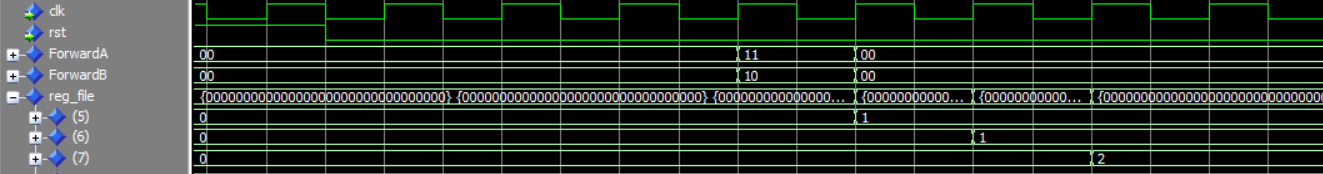
\includegraphics[width=1\textwidth]{sec3/images/wave_test5.png}
	\caption{Testing Forwarding of both data}
	\label{fig:wavetest5}
\end{figure}
\begin{figure}[H]
	\centering
	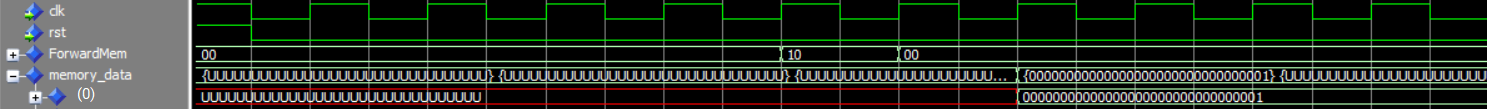
\includegraphics[width=1\textwidth]{sec3/images/wave_test6.png}
	\caption{Testing memory Forwarding}
	\label{fig:wavetest6}
\end{figure}

\subsection{Testing Load Hazard}
This script checks the operation of the hazard detection unit when a data dependency occurs that cannot be resolved by data forwarding.
\begin{figure}[H]
	\centering
	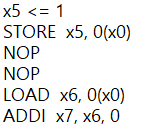
\includegraphics[width=0.2\textwidth]{sec3/images/test7.png}
	\caption{Testing Load Hazard}
	\label{fig:test7}
\end{figure}
\noindent In this case there is a load hazard between the LOAD operation and the ADD Immediate because the output register of the former coincides with the source address of the latter. The LOAD instruction retrieves the data from memory and saves it in the register, so the data will only be visible in the MEM stage. The addition operation, on the other hand, requires the data during the Execute stage, so even though it is forwarding, the hazard would not be eliminated. Then the hazard detection unit operates as if there were a control hazard, i.e. inserting two NOPs but without updating the PC, which remains at the current value in order to pick up again the pointed instruction since it has been flushed. In this way the drawback corresponds to two instructions, although through optimisation it could be reduced to one. In order not to increase the complexity of the machine, the solution described above has been chosen.\\
The \autoref{fig:wavetest7} shows how the registers are set to NOP and the PC remains set to the current value as soon as the load hazard is detected.
\begin{figure}[H]
	\centering
	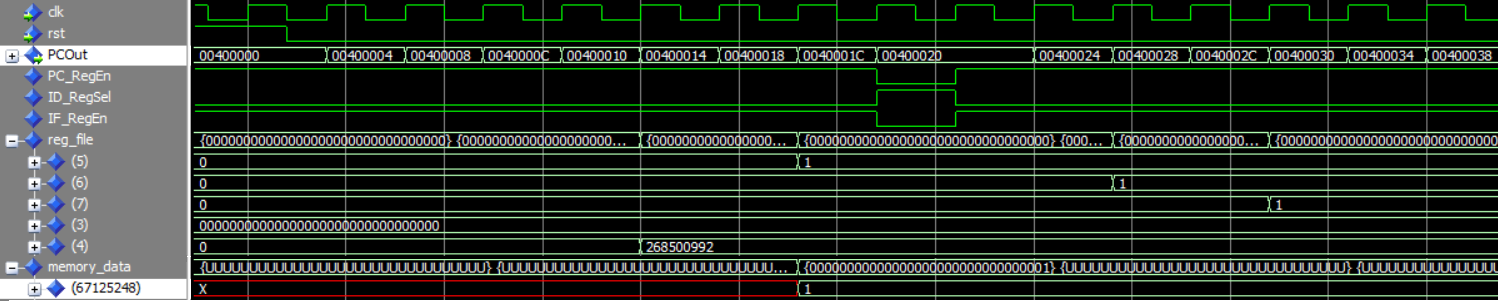
\includegraphics[width=1\textwidth]{sec3/images/wave_test7.png}
	\caption{Testing Load Hazard}
	\label{fig:wavetest7}
\end{figure}

\subsection{Testing a complete program}
This application searches for the smallest number in absolute value within a vector and saves the result in memory.
\begin{figure}[H]
	\centering
	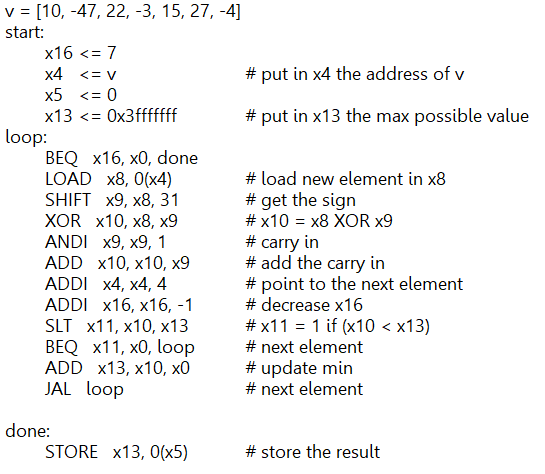
\includegraphics[width=0.6\textwidth]{sec3/images/test8.png}
	\caption{Testing Load Hazard}
	\label{fig:test8}
\end{figure}
\noindent Starting from a vector of 7 elements saved in memory, the algorithm takes one element of the vector from memory each time and compares it with the current minimum. If it finds a new minimum, then it is updated, otherwise it continues. When the whole vector has been analysed, the minimum is saved in memory. Since there is no instruction in the ISA that evaluates the absolute value of a number, the operations are slightly more complicated because the positive value has to be executed first using 3 instruction rather then one. The optimised code with the extended ISA can be found in the \autoref{subs:testAbs}.
The figure shows the seven executions of the cycle and the correct minimum research.\todo{insert figure}

\subsection{Testing Absolute Value Instruction}
\label{subs:testAbs}
To test the correct operation of the new RISC-V with the extended ISA thanks to the addition of the absolute value instruction, the same algorithm as in the previous subsection can be used, slightly modifying the code.
\begin{figure}[H]
	\centering
	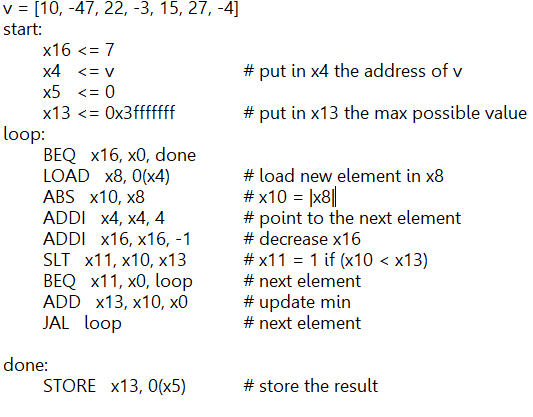
\includegraphics[width=0.6\textwidth]{sec3/images/test9.png}
	\caption{Testing Load Hazard}
	\label{fig:test9}
\end{figure}
\noindent The operation is identical to the previous case, but the cycle lasts fewer clock cycles and therefore the algorithm in general takes less time. The result is no different from the previous one.